\documentclass[12pt]{report}
\usepackage[T1]{fontenc}
\usepackage[utf8]{inputenc}
\usepackage{graphicx}
\usepackage{wrapfig}
\usepackage{amsmath,amssymb,amsfonts}
\usepackage{txfonts}
\usepackage{placeins}
\usepackage{listings}
\usepackage{pdfpages}
\usepackage{color}
\usepackage{framed}
\usepackage{filecontents}
\usepackage{caption}

\makeatletter
% --------------------------------------- C++
\let\oldaddcontentsline\addcontentsline
\newcommand{\lstlistcplusplusname}{List of C++}
\lst@UserCommand\lstlistofcplusplus{\bgroup
    \let\contentsname\lstlistcplusplusname
    \let\lst@temp\@starttoc \def\@starttoc##1{\lst@temp{loc}}%
    \tableofcontents \egroup}
\newcommand{\lstinputcplusplus}[2][]{{%
  \renewcommand{\lstlistingname}{C++ Code}%
  \renewcommand{\addcontentsline}[3]{\oldaddcontentsline{loc}{##2}{##3}}%
  \lstinputlisting[language=C++,breaklines=true,#1]{#2}%
}}

\usepackage[polish]{babel}

\renewcommand{\chaptername}{Rozdział}
\renewcommand{\contentsname}{Spis treści}
\renewcommand{\figurename}{Rys.}
\renewcommand{\tablename}{Tab.}
\renewcommand{\listfigurename}{Spis rysunków}
\renewcommand{\listtablename}{Spis tabel}
\renewcommand{\bibname}{Bibliografia}

\pagestyle{headings}

\setlength{\textwidth}{14cm}
\setlength{\textheight}{20cm}

\begin{document}

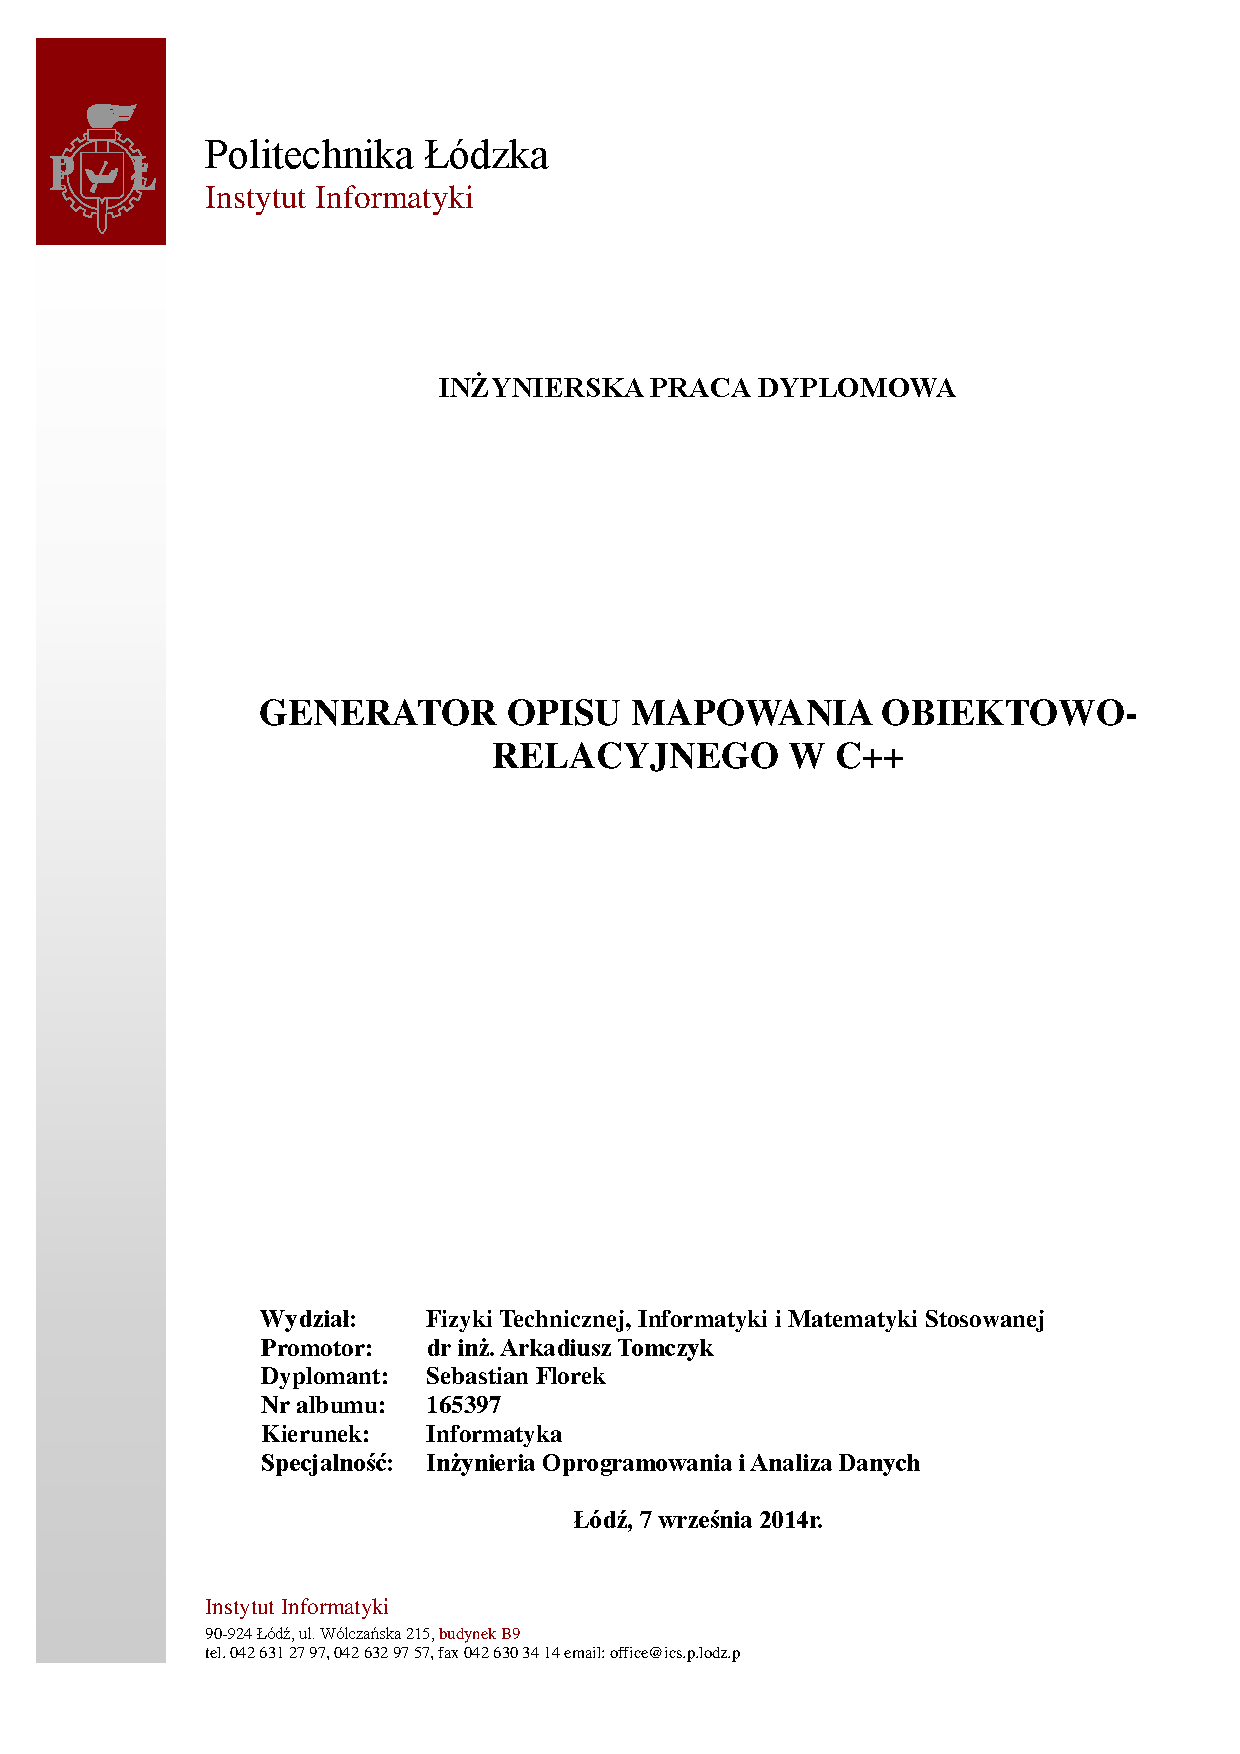
\includepdf[pages={1}]{images/title_page.pdf}

\tableofcontents	% generuje spis treści ze stronami !!!

\chapter{Wstęp}\label{chap:wstep} 

\section{Problematyka i zakres pracy}
Wzorzec architektoniczny typu Model View Controller
	\footnote{Model View Controller (MVC) - wzorzec służący do organizowania struktury aplikacji \cite{mvc}.}
jest obecnie szeroko używany przy projektowaniu aplikacji. Implementacja modelu warstwy danych w
rozbudowanych aplikacjach opartych o bazy danych jest czasochłonna i kosztowna. Rozwiązaniem tego
problemu jest zlecenie generowania warstwy danych aplikacji zewnętrznej. \\
	\indent Patrząc na średniej wielkości bazę danych z 30 tabelami, po 5 wierszy na tabelę,
człowiek musiałby napisać 30 klas po minimum 80 linijek każda, co przekłada się na 2400 linii kodu. 
Oszczędność czasu, a co za tym idzie i pieniędzy, przy zleceniu tego zadania programowi jest ogromna,
również szansa popełnienia błędu maleje znacząco, zakładając spełnienie przez użytkownika
kryteriów narzuconych przez tego typu aplikacje. \\
	\indent Narzędzia czy aplikacje szkieletowe służące do mapowania obiektowo-relacyj\-nego
	\footnote{Mapowanie Obiektowo-Relacyjne (ang. ORM, Object Relational Mapping) - przedstawia sposób odwzorowania obiektowej architektury
	systemu informatycznego na bazę danych lub inny element systemu o relacyjnym charakterze \cite{hibernateInAction}.}
używane przez programistów muszą być zazwyczaj dopasowywane do ich potrzeb. Pozwalają one zachować połączenie między bazą
danych, a ich systemem. W fazie deweloperskiej cyklu produkcji można zauważyć, że procesy projektowania i implementacji warstwy danych są bardzo podobne, co za tym idzie,
stają się one rutynowymi zadaniami cyklu produkcyjnego. \\
	\indent Po zbadaniu obecnie dostępnych narzędzi służących do mapowania obiektowo-relacyjnego
można znaleźć pewne wzorce i programy służące do generowania warstwy danych aplikacji, m. in.: {\color{black} aplikacje takie jak Hibernate czy JOOQ stworzone w języku Java lub QxEntityEditor napisany w języku C++}, jednakże ich niska skuteczność i wydajność związane z wieloma zapytaniami do bazy oraz czasem konfiguracji sprawiają, że szukamy czegoś innego.
{\color{black} Większość tego typu narzędzi bardziej skupia się na udostępnieniu jak największej funkcjonalności, przez co zanied\-bują warstwę danych,
która jest bardzo ważnym komponentem i najniższą warstwą aplikacji opartych o bazy danych.} \\
	\indent Głównym problemem staje się więc stworzenie warstwy danych, która zapewni bezpieczeństwo, wydajność oraz będzie optymalna, a następnie generatora, który pozwoli zautomatyzować ten proces. W przeciwieństwie do większości istniejących narzędzi, które generują bazę danych na podstawie istniejącej warstwy danych aplikacji,
nasza aplikacja będzie generowała warstwę danych aplikacji w oparciu o istniejącą bazę danych. \\
	\indent Proponowanym rozwiązaniem powyższych problemów będzie zaprojektowana aplikacja o nazwie Qubic. Dzielić ona będzie główną warstwę danych
na mniejsze warstwy na podstawie istniejącej bazy danych. Kluczem jest pozwolenie innym deweloperom na prace z konkretnymi obiektami, bez praktycznej znajomości
języków typu SQL
	\footnote{SQL (ang. Structured Query Language) - język programowania stworzony do zarządzania danymi, które trzymane są w relacyjnych bazach danych \cite{sql}.} 
 do obsługi baz danych. \\
	\indent Aplikacja została podzielona na dwa moduły i będzie tworzona przez dwie osoby. Pierwszy moduł będzie zajmował się generowaniem opisu relacyjnej bazy danych w postaci plików klas języka C++ i zostanie opisany w niniejszej pracy. Moduł generatora opisu mapowania obiektowo-relacyjnego będzie udostępniony jako biblioteka współdzielona. Dzięki takiemu rozwiązaniu moduły będą mogły być używane niezależnie. Drugi moduł zostanie opisany przez kolegę Marcina Maciaszczyka w pracy pod tytułem: ,,Mapowanie Obiektowo-Relacyjne w języku C++''.  Będzie on zajmował się procesem mapowania 
obiektowo-relacyjnego wygenerowanych klas na obiekty baz danych i udostępniał
odpowiednie interfejsy do obsługi operacji  zapisu i odczytu na bazie danych.

\section{Metoda badawcza}
\begin{enumerate}
\item Studia literaturowe z dziedziny generowania opisu mapowania obiektowo-relacyjnego w języku C++. \\ \\
Obecnie dostępne źródła z tej dziedziny nie są sformalizowane. Dostępne są jedynie opisy i dokumentacje istniejących aplikacji, które uwzględniają
w sposób ogólny ich budowę. Znalezione i użyte w tej pracy źródła nie są dostępne w języku polskim, więc muszą być tłumaczone w większości z języka angielskiego.
Jako że nie ma oficjalnych książek dotyczących tematyki generowania opisu mapowania obiektowo-relacyjnego, większość źródeł tu zebranych to źródła elektroniczne, artykuły i dokumentacje.
\item Analiza wymagań aplikacji szkieletowych generujących opis mapowania obie\-ktowo-relacyjnego. \\ \\
Narzędzia zajmujące się generowaniem opisu mapowania obiektowo-relacyj\-nego są zazwyczaj tylko dodatkami do typowych aplikacji typu ORM. Nie znajdziemy tu
modelu aplikacji, na którym można bazować. Wymagania postawione takiej aplikacji są zazwyczaj takie same i są one podyktowane przez aplikacje zajmujące się mapowaniem obiektowo-relacyjnym. Podobnie jest i w tym przypadku gdzie wymagania generatora opisu są postawione przez drugi moduł aplikacji zajmujący się mapowaniem obiektowo-relacyjnym.
\item Proces projektowania i tworzenia Qubica. \\ \\
W oparciu o zebrane informacje i wymagania aplikacji szkieletowych służą\-cych do generowania opisu mapowania obiektowo-relacyjnego zostanie stworzona aplikacja szkieletowa mająca na celu rozwiązanie problemów zidentyfikowanych w procesie analizy.
\item Testy i wnioski dotyczące stworzonego narzędzia do generowania warstwy danych aplikacji w oparciu o bazę danych. \\ \\
Metoda ta służy do wyciągnięcia wniosków na temat stworzonej aplikacji. Przeprowadzone zostaną testy porównawcze. Na podstawie wyników testów wyciągnięte zostaną odpowiednie wnioski na temat sposobu rozwiązania przedstawionych w pracy problemów oraz Qubica. Wszystko to pozwoli stwierdzić czy proponowane rozwiązanie jest lepsze, tańsze, szybsze od porównywanych.

\end{enumerate}

\section{Przegląd literatury w dziedzinie}
\subsubsection{Źródła z zakresu języka C++}
	\indent Użyte w tej pracy źródła dotyczące języka C++ służą przede wszystkim poznaniu technik programowania bibliotek współdzielonych oraz technik metaprogramowania. Dodatkowym celem przy pisaniu samej aplikacji jest chęć poznania nowego standardu języka C++11, który również jest przedstawiony w użytych źródłach. Szczegółowe omówienie tego standardu zostało przedstawione na stronie twórcy języka i służyć będzie jako główne źródło wiedzy \cite{strostrup}.
Sposób tworzenia bibliotek i techniki metaprogramowania zostały opisane w książce Advanced C++ Metaprogramming \cite{c++2}.
\subsubsection{Źródła z zakresu narzędzi i aplikacji do mapowania obiektowo-relacyjnego}
	\indent Tematyka generowania opisu mapowania obiektowo-relacyjnego jest związana z narzędziami ORM i brak jest książek dedykowanych tej tematyce. Do zrozumienia samej idei działania generatora należy przybliżyć działanie narzędzi do mapowania obiektowo-relacyjnego. W pozycjach EJB 3 Java persistence API \cite{ejb} oraz Hibernate w akcji \cite{hibernateInAction}
znajdziemy opis działania narzędzi typu ORM oraz techniki mapowania obiektowo-relacyjnego.
\subsubsection{Źródła z zakresu działania aplikacji szkieletowej Qt}
	\indent Aplikacja szkieletowa Qt to zestaw bibliotek i narzędzi przydatnych programistom. Dzięki mechanizmowi refleksji, wsparciu dialektów SQL czy prostej budowie aplikacji graficznych znacznie ułatwia tworzenie dużych aplikacji. Użyta książka Introduction to Design Patterns in C++ with Qt \cite{c++patterns}
opisuje w prosty sposób mechanizm refleksji, wzorce czy tworzenie bibliotek przy użyciu tego frameworka.
Dodatkowo głównym narzędziem w etapie tworzenia aplikacji będzie dokumentacja Qt dostępna w internecie pod adresem \cite{qtframework}.
\subsubsection{Źródła z zakresu SQL}
	\indent W celu generowania opisu bazy danych potrzebna jest znajomość struktury bazy, typów pól, połączeń. Wymaga to dla niektórych dialektów SQL pisania dość nietypowych zapytań. Potrzebne informacje zostały zasięgnięte ze źródeł elektronicznych i odpowiednich dokumentacji konkretnych dialektów, m. in: stron internetowa z dokumentacją dialektu MySQL \cite{mysqlweb}.



\section{Układ pracy}
Tematem pracy jest stworzenie generatora opisu mapowania obiektowo-relacyjnego w C++, zaś za główny cel przyjęto rozwiązanie problemu
automatycznego generowania warstwy danych w aplikacjach opartych o relacyjne bazy danych. \\
Rozdział \ref{chap:wstep} zawiera szczegółowy opis problemu. {\color{black} Przedstawione są w nim różne problemy związane z aplikacjami generującymi warstwę danych aplikacji},
wraz z opisem metod badawczych użytych do analizy tematu. Podsumowane zostają również główne założenia i cele pracy.
Na koniec przeprowadzony zostaje przegląd literatury z dziedziny generowania opisu mapowania obiektowo-relacyjnego. Zostają w nim wyróżnione
najważniejsze {\color{black} zagadnienia} dotyczące prezentowanego tematu wraz z krótkim opisem użytych źródeł.  \\
W rozdziale \ref{chap:generator} przybliżona zostaje tematyka tworzenia aplikacji opartych o warstwy. Znajduje się tam opis warstwy dostępu do danych, która musi zostać wygenerowana. Następnie po kolei przedstawione zostają tematyki związane z bazami danych, mapowaniem obiektowo-relacyjnym oraz użytymi wzorcami projektowymi. Na końcu znajduje się opis sposobu działania bibliotek współdzielonych oraz aplikacji szkieletowej Qt. \\
Rozdział \ref{chap:analiza} zawiera analizę istniejących aplikacji służących do generowania opisu mapowania obiektowo-relacyjnego. Wymienione zostają same aplikacje, wspierane systemy, opisane zostają ich słabe i mocne punkty. \\
Kolejny rozdział opisuje fazę projektowania i implementacji aplikacji Qubic. Spisane są wymagania funkcjonalne aplikacji, a także ograniczenia projektu. Przybliżony zostaje projekt w postaci diagramów klas.\ Pokazane zostaje wykorzystanie wzorców projektowych na etapie tworzenia aplikacji. Wskazane zostają kluczowe punkty aplikacji wraz z kodem źródłowym i opisem. Następnie następuje faza testów stworzonej aplikacji oraz zestawienie i porównanie wyników testów podobnych aplikacji. \\
W podsumowaniu pracy przedstawiono uzyskane w fazie testowania wyniki stworzonej aplikacji. Opisane zostają zrealizowane cele, słabe i mocne punkty przedstawionego rozwiązania.\ Na podstawie wyników następuje ocena możliwości i przydatności zaproponowanego rozwiązania. Na końcu omówione zostają możliwe perspektywy rozwoju generatora opisu mapowania obiektowo-relacyjnego.

\chapter{Generator opisu mapowania obiektowo-relacyjnego w C++}\label{chap:generator}
\chaptermark{Generator opisu w C++}
\section{Podstawowe definicje}
Użyte koncepcje i terminy używane w dalszej części pracy muszą zostać wyjaśnione w celu lepszego zrozumienia opisywanej problematyki. W kolejnych rozdziałach zostają objaśnione podstawowe pojęcia związane z tematyką generowania opisu mapowania obiektowo-relacyjnego w C++. Są opisane terminy związane z bazami danych, aplikacjami z zakresu ORM, wzorcami projektowymi, aplikacjami zajmującymi się generowaniem kodu. Na koniec przybliżone zostają biblioteki współdzielone oraz framework Qt użyty przy tworzeniu części praktycznej tej pracy.
\subsection{Warstwa dostępu do danych}
	\indent Warstwa dostępu do danych aplikacji jest najniższą warstwą w architekturze aplikacji. Jej głównym zadaniem jest stworzenie mostu pomiędzy bazą danych, a samą aplikacją, tak aby możliwe było wykonywanie podstawowych operacji na bazie danych z poziomu aplikacji, tj. odczytu, zapisu oraz tworzenia i usuwania rekordów. W programowaniu, warstwa danych służy zwróceniu referencji obiektu wraz z jego atrybutami, gdzie klasa odpowiada tabeli w bazie danych, a jego atrybuty odpowiednim kolumnom tej tabeli. \\
	\indent Aplikacje używające warstwy dostępu do danych mogą być zależne lub niezależne od bazy danych. Jeśli warstwa dostępu do danych wspiera wiele typów baz danych, aplikacja staje się bardziej generyczna. Ułatwia to przystosowanie aplikacji do innego typu baz danych bez dużego wysiłku. Zazwyczaj jest to realizowane poprzez nadpisanie odpowiednich klas. Tego typu praktyki są stosowane często właśnie w narzędziach zajmujących się mapowaniem obiektowo-relacyjnym \cite{datalayer}.
\subsection{Normalizacja bazy danych}
	\indent Normalizacja bazy danych jest procesem organizacji tabel oraz ich pól w relacyjnych bazach danych, w taki sposób aby zminimalizować redundancję danych. Proces ten zazwyczaj ma na celu zdefiniowanie połączeń między tabelami, a następnie ich podział na mniejsze logiczne części, które zmniejszą powtarzalność danych w bazie \cite{sql}.
\subsection{SQL}
	\indent SQL jest językiem programowania stworzonym do zarządzania danymi, które są trzymane w relacyjnych bazach danych. Głównym zadaniem tego języka jest dodawanie, usuwanie, odczyt oraz aktualizacja danych. Na bazie języka SQL zostało stworzonych wiele systemów zarządzania relacyjnymi bazami danych oraz nowych dialektów SQL, które są obecnie powszechnie używane. Jednym z takich systemów zarządzania relacyjnymi bazami danych jest MySQL, który został użyty jako główny system przy projektowaniu i implementacji części praktycznej tej pracy \cite{sql}.
\subsection{Mapowanie Obiektowo-Relacyjne}
	\indent Mapowanie obiektowo-relacyjne jest techniką programowania używaną w celu konwersji danych pomiędzy niekompatybilnymi systemami. Rozwiązaniem problemu różnej budowy tych systemów jest stworzenie w pamięci programu wirtualnej bazy danych obiektów, które mogą być używane bezpośrednio przez aplikacje \cite{hibernateInAction}.\ Obie\-kty przebywające w pa\-mięci muszą być powiązane z danymi w bazie danych.\ Tabele relacyjnej bazy danych mają swoje odwzorowanie w obiektach języka programowania. Tworzone są one na podstawie metadanych opisujących to odwzorowanie. Mapowanie obiektowo-relacyjne musi być zatem procesem dwukierunkowym, tak aby obie strony relacji operowały zawsze na aktualnych danych. Samo rozwiązanie mapowania składa się z czterech elementów:
	\begin{itemize}
	\item{interfejsu do przeprowadzania podstawowych operacji CRUD na obiektach klas zapewniających trwałość}
	\item{języka lub interfejsu programistycznego do określania zapytań związanych z klasami lub ich właściwościami}
	\item{narzędzia do określania metadanych}
	\item{technik implementacji ORM, zachowujących integralność między obiektami}
	\end{itemize}

	\begin{figure}[!ht]
		\centering
		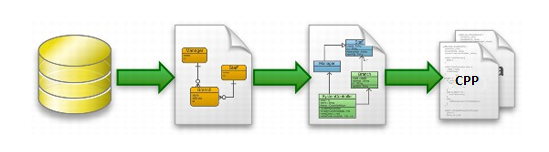
\includegraphics[width=1\textwidth]{images/orm.png}
		\caption{Uproszczony przebieg generowania opisu mapowania obiektowo-relacyjnego \cite{ormimg}.}
	\end{figure}

\subsection{Wzorzec projektowy}
	\indent {\color{black} Wzorce projektowe są wydajnym i eleganckim sposobem na rozwiązanie najczęściej spotykanych problemów przy tworzeniu aplikacji obiektowych. Zostały one spopularyzowane dzięki twórcom książki ,,Inżynieria oprogramowania: Wzorce projektowe''. Erich Gamma, Richard Helm, Ralph Johnson oraz John Vlissides nazywani także ,,Bandą Czterech'' przeanalizowali w niej 23 wzorce \cite{c++patterns}.}   Pozwalają one na wyodrębnienie często używanych części algorytmów, tak aby mogły być używane przez różne części systemu. Nie są to gotowe rozwiązania, a jedynie opisy oraz szablony zawierające wskazówki rozwiązania tych samych problemów występujących w różnych sytuacjach. \\
	\indent Wzorce programowania obiektowego zazwyczaj pokazują relacje i powiązania pomiędzy obiektami bez specyfikacji tych obiektów. Są one stosowane na poziomie projektowania aplikacji. \\
	\indent Typy wzorców projektowych możemy podzielić na:
	\begin{itemize}
		\item{Wzorce konstrukcyjne - opisujące proces tworzenia nowych obiektów. Ich zadaniem jest tworzenie, inicjalizacja oraz konfiguracja obiektów.}
		\item{Wzorce strukturalne - opisujące struktury powiązanych ze sobą obiektów.}
		\item{Wzorce czynnościowe - opisujące zachowanie i powiązania współpracujących ze sobą obiektów.}
	 \end{itemize} 
\subsection{Wzorzec architektoniczny Model-Widok-Kontroler}
	\indent Wzorzec architektoniczny model-widok-kontroler oddziela od siebie warstwy: do\-stępu do danych, kontrolera oraz widoku. Każda warstwa odpowiada za inne zadania.
	\begin{itemize}
	\item Warstwa modelu - zarządza dostępem do danych oraz wszelkimi zmianami z nimi związanymi
	\item Warstwa kontrolera - interpretuje sygnały płynące z warstwy widoku. Informuje warstwy dostępu do danych oraz widoku o wymaganych zmianach.
	\item Warstwa widoku - zarządza wyświetlaniem informacji. 
	\end{itemize}
Przykładowy obrazek przedstawia w prosty sposób schemat działania tego wzorca oraz przepływ informacji między warstwami. \\
\begin{figure}[h]
	\centering
	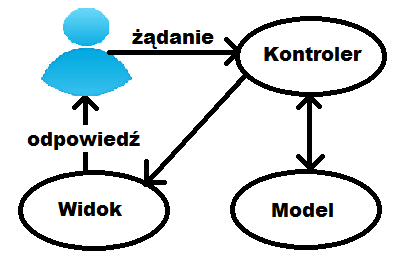
\includegraphics[width=0.6\textwidth]{images/mvc.png}
	\caption{Wzorzec Model-Widok-Kontroler.}
\end{figure}
\FloatBarrier
\subsection{Komponent Data Access Object}
	\indent Data Access Object jest komponentem, którego zadaniem jest dostarczanie jednolitego interfejsu do komunikacji między aplikacją, a źródłem danych(np. bazą danych czy plikiem). Dostarcza on możliwość manipulacji danymi bez wykonywania bezpośrednich operacji na źródle danych, a jedynie na obiekcie. Głównymi zaletami takiego podejścia są prostota użycia i czytelność. Zmiana logiki nie wymaga zmian w źródle danych i na odwrót. Pozwala to również ukryć szczegóły związane ze źródłem danych oraz w łatwy sposób zmienić je w razie potrzeby \cite{dao}.
\subsection{Biblioteka współdzielona}
	\indent Biblioteka współdzielona jest ładowana tylko raz do pamięci systemu. Każdy proces który załaduje taka bibliotekę do własnej pamięci procesu jedynie mapuje adresy do oryginalnych wywołań funkcji. W przeciwieństwie do bibliotek statycznych kod funkcji nie jest kopiowany do pamięci procesu, który je wywołuje. Przechowywane są jedynie wirtualne adresy funkcji do których odwołuje się proces. Raz załadowana biblioteka współdzielona może być więc używana przez wiele procesów jednocześnie co zmniejsza zużycie pamięci \cite{dll}.
\begin{figure}[h]
	\centering
	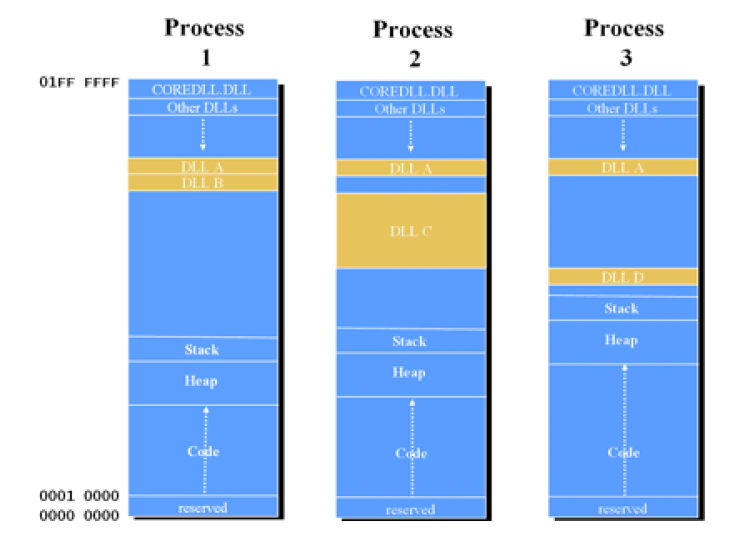
\includegraphics[width=.8\textwidth]{images/dll.png}
	\caption{{\color{black} Schemat działania biblioteki współdzielonej \cite{dllimg}.}}
\end{figure}
\FloatBarrier
\subsection{Aplikacja szkieletowa Qt}
	\indent Aplikacja szkieletowa Qt jest gotowym narzędziem skierowanym do programistów C++, jak również osób preferujących język CSS i Javascript do budowania aplikacji. Posiada moduły potrzebne do budowy kompletnej aplikacji, m. in.:
	\begin{itemize}
	\item Biblioteki języka C++ przeznaczone na wiele platform
	\item Wsparcie dla budowania interfejsu użytkownika przy użyciu różnych narzędzie
	\item Zintegrowane środowisko deweloperskie
	\end{itemize}
	\indent Główną zaletą używania Qt jest możliwość pisania kodu skierowane pod wiele platform. Moduły obsługi bazy danych, budowy interfejsu użytkownika i wiele innych pozwalają znacznie skrócić czas potrzebny na tworzenie aplikacji. Jest również jednym z niewielu narzędzi w języku C++, które bardzo dobrze wspiera refleksję\footnote{{\color{black}Mechanizm refleksji - pozwala na modyfikację działania programu w trakcie jego wykonania. Zachowanie funkcji lub metod wcześniej zdefiniowanych może ulec zmianie w trakcie działania programu.}} \cite{qtframework}.

\chapter{Analiza istniejących aplikacji do generowania opisu mapowania obiektowo-relacyjnego}\label{chap:analiza}
\chaptermark{Analiza istniejących aplikacji}
W tym rozdziale zostaną przeanalizowane istniejące aplikacje zajmujące się generowaniem opisu mapowania obiektowo-relacyjnego. Sprawdzone zostaną ich słabe i mocne stron oraz wymagania.
\section{Istniejące aplikacje}
\indent W języku C++ liczba aplikacji zajmujących się generowaniem opisu mapowania obiektowo-relacyjnego jest znikoma. Jedyna warta uwagi biblioteka to QxORM, a w zasadzie specjalny generator zbudowany na jej podstawie o nazwie QxEntityEditor. W języku Java istnieje kilka aplikacji zajmujących się generowaniem opisu mapowania obiektowo-relacyjnego. Są nimi: JOOQ \cite{jooqweb} czy Hibernate \cite{hibernateweb}. Obie aplikacje zajmują się mapowaniem obiektowo-relacyjnym i posiadają funkcjonalność generowania warstwy dostępu do danych z istniejących systemów relacyjnych baz danych.
\section{Wymagania aplikacji}
W przeciwieństwie do analizowanych aplikacji Javowych QxEntityEditor został stworzony jako całkowicie niezależna aplikacja, jednak aby generowanie kodu było możliwe wymaga on dostępu do biblioteki QxORM. Pozostałe aplikacje, tj. JOOQ oraz Hibernate zostały stworzone przy użyciu języka Java. Dzięki temu mogą one być używane zarówno na systemach unixowych, jak i tych z rodziny Windows. Sam Hibernate nie posiada opcji generowania modelu warstwy danych aplikacji. Dostępne są w tym celu odpowiednie wtyczki do środowisk programistycznych, takich jak Eclipse czy Intellij. Aplikacja JOOQ natomiast rozwiązała ten problem i udostępnia funkcję generatora kodu z linii poleceń.
Jedynym wymogiem oprócz posiadania odpowiedniego środowiska, z którego wygenerowany zostanie projekt na podstawie bazy danych, jest stworzenie odpowiedniego pliku konfiguracyjnego.

\section{Hibernate}
Hibernate udostępnia możliwość mapowania modelu danych na relacyjną bazę danych. Dostarcza on również dodatkowe narzędzia, które pozwalają ten proces odwrócić. Są to odpowiednie wtyczki do środowisk programistycznych takich jak Eclipse czy IntelliJ. Udostępniony interfejs jest prosty w obsłudze, a konfiguracja wymaga jedynie dostarczenia odpowiedniego pliku z informacjami o połączeniu. Wadą jest niestety brak możliwości zdefiniowania przez użytkownika dodatkowych informacji, np. dotyczących relacji między tabelami. Dużym plusem jest to, że wszystkie te narzędzia są dostępne za darmo na licencji LGPL\footnote{LGPL - licencja wolnego oprogramowania. Pozwala między innymi na używanie oprogramowania objętego taką licencją w komercyjnych projektach, bez konieczności zakupu licencji.}

\begin{figure}[h]
	\centering
	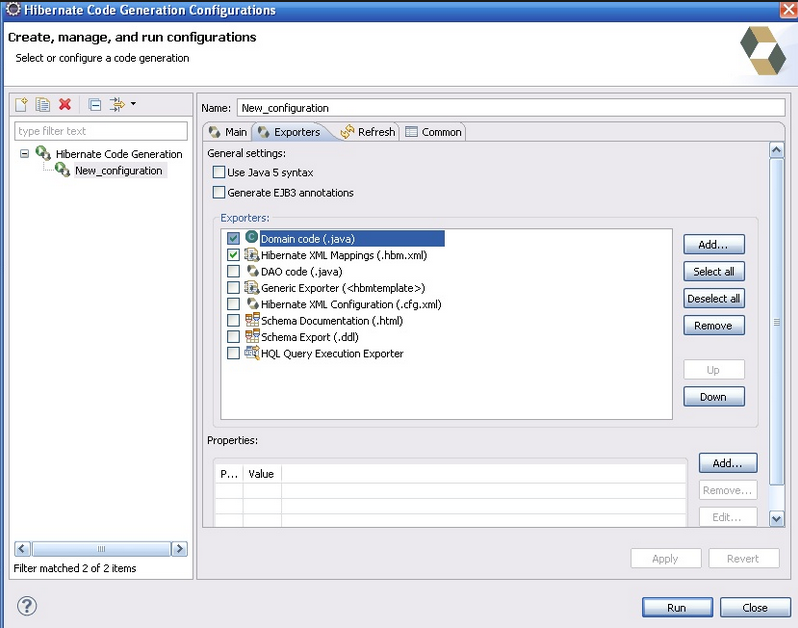
\includegraphics[width=.67\textwidth]{images/eclipse.png}
	\caption{Interfejs generowania kodu frameworka Hibernate.}
\end{figure}

\FloatBarrier

\section{JOOQ}
Jest stosunkowo nowym i lekkim narzędziem do mapowania obiektowo-relacyjnego. Głównym założeniem twórców było postawienie SQL na pierwszym miejscu. Zamiast tworzyć własny język do generowania zapytań, skupili się na prostym i szybkim generowaniu zapytań SQL. Nie udostępnia on dużej funkcjonalności jak na przykład Hibernate jednak dzięki temu oferuje szybkość i prostotę użycia. Generowanie kodu odbywa się niestety z linii poleceń, jako że nie udostępnia on żadnego graficznego interfejsu. Generowanie odbywa się jednostronnie, czyli z istniejącej bazy danych do projektu języka Java. W celu wygenerowania projektu należy przygotować wcześniej odpowiedni plik ustawień i wywołać odpowiednią klasę.

\begin{framed}
\centering
\begin{lstlisting}[language=Java]
java org.jooq.util.GenerationTool /jooq-config.xml
\end{lstlisting}
\end{framed}

\FloatBarrier

Niestety biblioteka JOOQ w darmowej ofercie ma dość ograniczone możliwości. W celu uzycia jej do średnich i większych projektów wymagane jest wykupienie wersji profesjonalnej lub dla firm. W darmowej wersji nie obsługuję ona zbyt dużej ilości baz danych.

\section{QxEntityEditor}

QxEntityEditor jest graficznym edytorem przeznaczonym dla biblioteki QxORM. Pozwala on zarządzać modelem danych w bardzo szerokim zakresie, np.:

\begin{itemize}
\item{Pozwala generować klasy C++ na podstawie bazy danych przeznaczone do używania z biblioteką QxORM.}
\item{Pozwala generować skrypty tworzące bazę danych.}
\item{Wspomaga tworzenie aplikacji typu klient/serwer.}
\item{Udostępnia własny interfejs modelowania bazy danych. Nie wymaga jej wcześniejszego istnienia w celu stworzenia bazy oraz projektu.}
\end{itemize}

Użytkowanie aplikacji niestety nie jest zbyt proste ze względu na bardzo dużą funkcjonalność i dość niejasne błędy. Próby wygenerowania kodu z bazy MySQL niestety zakończyły się niepowodzeniem. Sama aplikacja jest płatna i nie udostępnia swoich źródeł co znacznie ogranicza jej dostępność dla zwykłego programisty.

\begin{figure}[h]
	\centering
	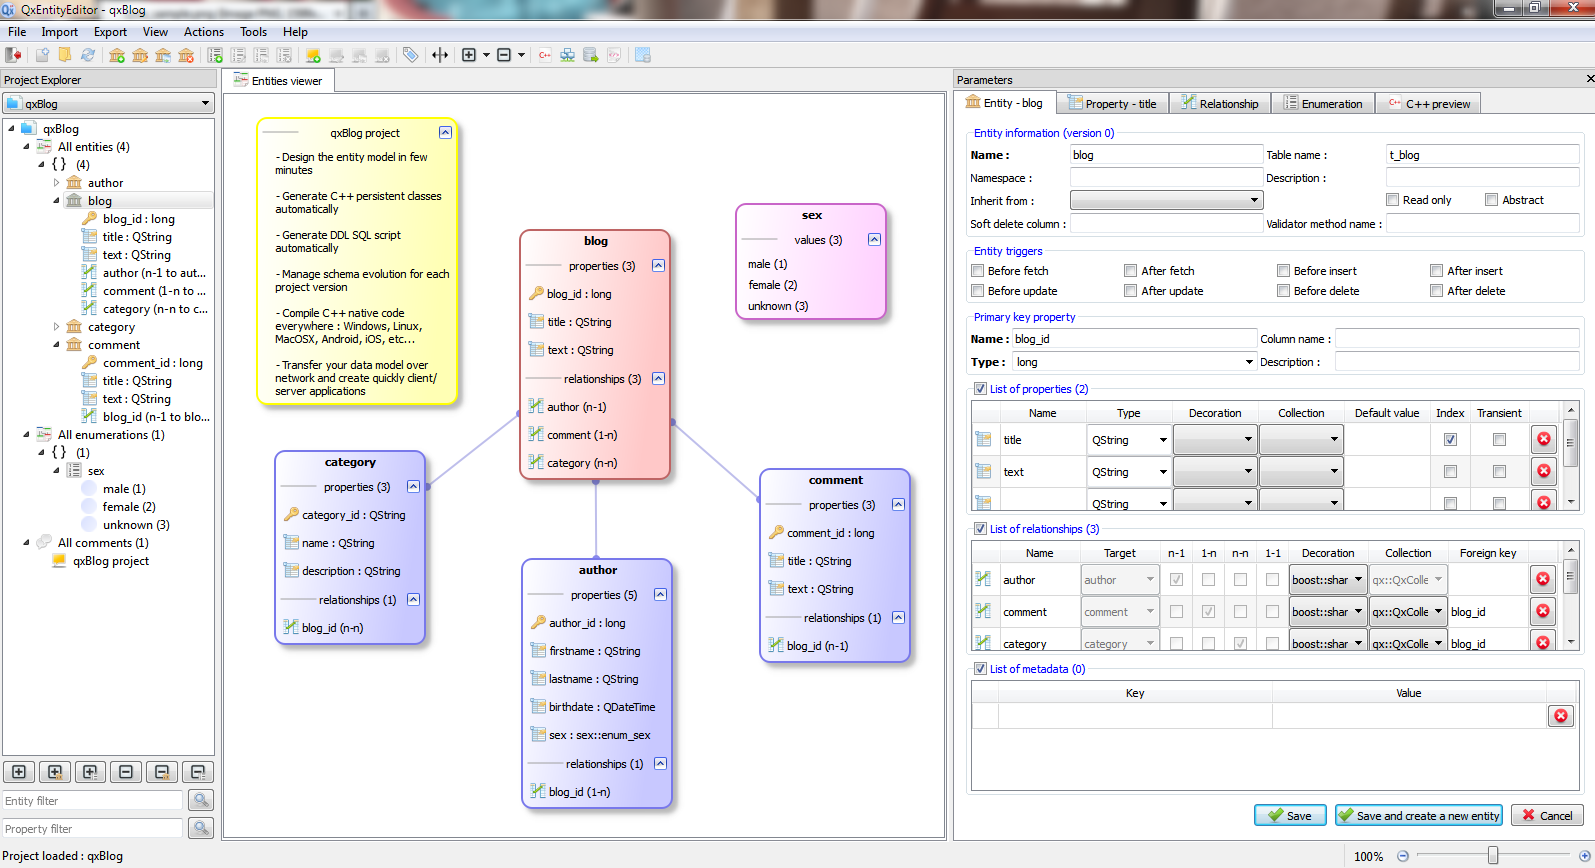
\includegraphics[width=1\textwidth]{images/qxentity.png}
	\caption{Interfejs aplikacji QxEntityEditor.}
\end{figure}

\FloatBarrier

\section{Wady i zalety istniejących rozwiązań}

\begin{table}[!ht]
\centering
    \begin{tabular}{| p{3cm} |  p{3cm} |  p{2cm} | p{3cm} |}
    \hline
    QxEntityEditor & JOOQ & Hibernate & \\ \hline
     tak & tak & tak & Wsparcie dla popularnych systemów baz danych \\ \hline
 duża & mała & duża & Dostępna funkcjonalność \\ \hline
 średnia & dobra & dobra & Przejrzystość generowanego kodu \\ \hline
 pojedyncza licencja 300\$ & od 320\$ do 640\$ w zależności od licencji & darmowy & Cena \\ \hline
 duży & średni & średni & Stopień trudności konfiguracji \\ \hline
    \end{tabular}
    \caption{Porównanie wybranych aplikacji zajmujących się generowaniem opisu mapowania obiektowo-relacyjnego.}
\end{table}

Podsumowując powyższą tabelę można stwierdzić, że każde z istniejących roz\-wiązań ma pewne wady lub braki. Z aplikacji przeznaczonych dla języka Java Hibernate jest zdecydowanym zwycięzcą jeśli chodzi o funkcjonalność, prostotę i cenę narzędzia do generowania opisu mapowania obiektowo-relacyjnego. JOOQ z drugiej strony swą prostotą użycia sprawia, że dla prywatnych użytkowników jest zdecydowanym liderem. Jeśli chodzi natomiast o język C++, tutaj jedynym kandydatem jest QxEntityEditor. Posiada on dużą funkcjonalność, jednak cena jaką należy zapłacić zdecydowanie odstrasza zwykłych użytkowników. Sprawia to, że staje się on narzędziem przeznaczonym raczej dla firm.

\chapter{Projekt aplikacji szkieletowej Qubic} \label{rozdz.czesc.prakt}

\section{Analiza wymagań}
	\indent W tej części zostanie przedstawiona analiza oraz część implementacyjna aplikacji Qubic. W pierwszej części są zdefiniowane wymagania aplikacji oraz opisane wymagania funkcjonalne wraz z ograniczeniami projektu. Następnie zostają przedstawione główne diagramy dotyczące działania aplikacji. Kolejna część opisuje technologie i metodologie użyte w projekcie z podziałem na warstwy modelu, widoku i kontrolera w aplikacji. Kolejna część zawiera przedstawienie proponowanego rozwiązania wraz z częścią implementacyjną. Przybliżone zostają najważniejsze części kodu wraz z opisem. Ostatnim krokiem są testy i ocena funkcjonalności stworzonej aplikacji.
\subsection{Studium możliwości}
	\indent Główną ideą projektu jest rozwiązanie problemu generowania warstwy dostępu do danych aplikacji. W celu minimalizacji zużycia pamięci oraz uzyskania jak najlepszej wydajności została stworzona jedna warstwa obiektów, gdzie każdy obiekt klasy odzwierciedla tabelę w bazie danych. Nie istnieje podział na obiekty transakcyjne i biznesowe. Aplikacja daje nam możliwość generowania warstwy dostępu do danych z większości obecnie istniejących systemów zarządzania relacyjnymi bazami danych.
\subsection{Wymagania funkcjonalne}
	\indent Ze względu na budowę własnego systemu mapowania obiektowo-relacyjnego moduł generowania danych musi spełniać pewne wymagania:
	\begin{enumerate}
	\item{Generowanie warstwy dostępu do danych w oparciu o relacyjne bazy danych.}
	\item{Generowanie plików klas oraz plików źródłowych.}
	\item{Generowane pliki powinny mieć czytelną i prostą budowę, aby były proste w użyciu dla programistów.}
	\item{Wszelkie ustawienia powinny być w prosty sposób konfigurowalne, tak by zmiana bazy danych nie wymuszała zmian kodu aplikacji.}
	\item{Powinna generować dodatkowe funkcje pozwalające wyciągnąć powiązane dane w oparciu o relacje między tabelami.}
	\item{Aplikacja powinna wspierać wiele systemów baz danych lub udostępniać łatwy sposób dodania ich wsparcia.}
	\item{Aplikacja powinna w prosty sposób definiować mapowanie typów danych z bazy danych na typy języka.}
	\end{enumerate}
\subsection{Ograniczenia projektu}
	\indent Ze względu na czytelność kodu oraz sposób działania modułu zajmującego się mapowaniem obiektowo-relacyjnym na bazę danych zostały nałożone pewne ograniczenia:
	\begin{itemize}
	\item{Każda tabela w bazie musi zawierać klucz główny.}
	\item{Każdy typ danych użyty w bazie musi zostać zarejestrowany w aplikacji i zmapowany na odpowiedni typ języka.}
	\item{Nazwy kolumn w tabelach mogą zawierać jedynie litery i cyfry ze względu na czytelność generowanego kodu.}
	\end{itemize}
	\indent Powyższe ograniczenia są rozpoznawane przez aplikację, a ich nie spełnienie wiąże się z brakiem możliwości generowania warstwy dostępu do danych. Kolejnym ograniczeniem jest brak integracji generatora z innymi aplikacjami do mapowania obiektowo-relacyjnego oraz współpraca jedynie z relacyjnymi bazami danych. Również błędne wskazanie relacji w tabelach może wiązać się z błędami logicznymi w wygenerowanym kodzie.
\section{Użyte technologie}
\subsection{Język programowania}
Do stworzenia aplikacji został wybrany język C++. Najważniejszym czynnikiem jego wyboru jest wydajność. W porównaniu podstawowych operacji między innymi popularnymi językami język ten jest zdecydowanie szybszy. Poniższa tabela przedstawia porównanie czasów wykonania: pętli, operacji tablicowych, podstawowych operacji matematycznych.
\begin{figure}[h]
	\centering
	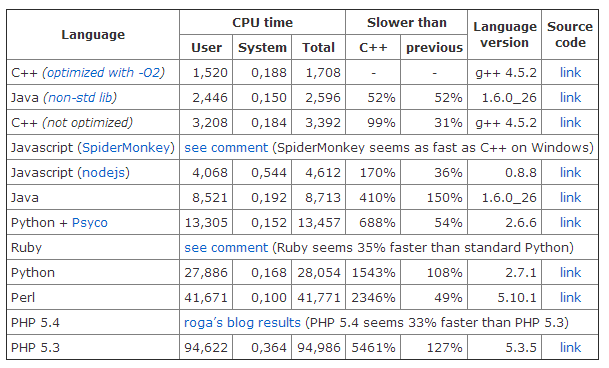
\includegraphics[width=1\textwidth]{images/c++test.png}
	\caption{Porównanie wydajności popularnych języków względem C++. \cite{c++testimg}}
\end{figure}
\FloatBarrier

Drugim ważnym czynnikiem wyboru języka C++ jest znikoma ilość aplikacji realizujących mapowanie obiektowo-relacyjne wraz z możliwością generowania warstwy dostępu do danych w tym języku.

\subsection{System baz danych}
Jako system zarządzania bazą danych został wybrany serwer MySQL. Czynniki które o tym zdecydowały to przede wszystkim mała zajętość pamięci oraz łatwa i szybka konfiguracja. Dodatkowo posiada on bardzo dobrą integrację z użytym frameworkiem Qt, który został użyty m.in.: w celu połączenia z bazą danych oraz odczytu jej struktury z poziomu języka C++.
\subsection{Środowisko deweloperskie}
Wybrane środowisko deweloperskie jest częścią użytego frameworka Qt. Qt Creator jest zintegrowany z zestawem bibliotek użytego frameworka i udostępnia wsparcie składni oraz informacje o interfejsie programowania aplikacji.
\subsection{Biblioteki}
Użyty zestaw bibliotek należy do frameworka Qt. Udostępnia on biblioteki przenośne i narzędzia programistyczne dedykowane dla języków C++, Java czy QML. Głównym atutem są klasy służące do budowy graficznego interfejsu użytkownika, wsparcie połączenia z wieloma systemami baz danych oraz obsługiwany mechanizm refleksji. Wszystkie te rzeczy w znacznym stopniu ułatwiają tworzenie aplikacji oraz skracają czas potrzebny na jej stworzenie.
\subsection{Inne narzędzia}

\begin{figure}[h]
	\centering
	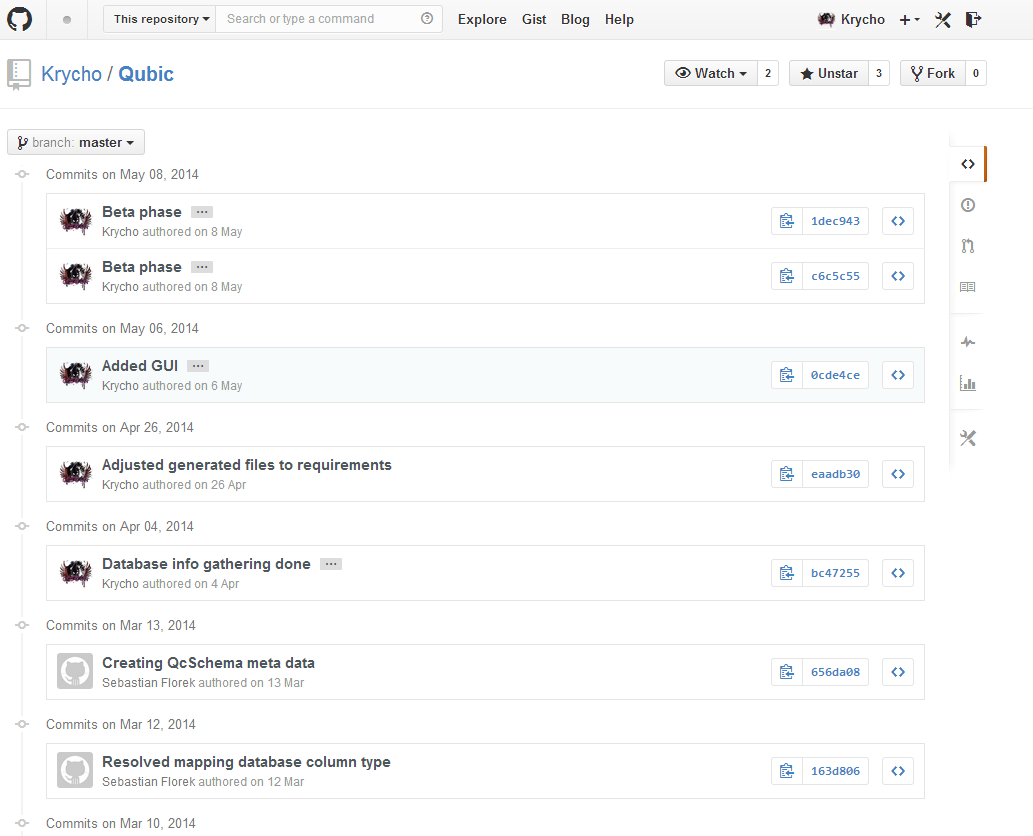
\includegraphics[width=.9\textwidth]{images/git.png}
	\caption{Log kontrolny zmian projektowych z portalu Github.}
\end{figure}
\FloatBarrier

Dodatkowym narzędziem użytym w procesie tworzenia aplikacji był system kontroli wersji o nazwie GIT. Pozwalało to kontrolować cały proces powstawania Qubica. Całość jest zintegrowana z portalem Github i przechowywana na prywatnym repozytorium.

\section{Projekt}
\subsection{Projekt warstwy danych}\label{sec:database}
\indent Poniżej przedstawiony kod został użyty do budowy {\color{black} testowej} bazy danych. Baza zawiera najważniejsze relacje potrzebne do testów tworzonej aplikacji, tj. jeden do wielu oraz wiele do wielu.
\begin{framed}
\lstinputlisting[language=SQL]{additional/database.sql}
\end{framed}

Użytkownik bazy danych, który posłuży nam do ustanowienia połączenia musi posiadać uprawnienia do odczytu informacji z tabel opisujących budowę bazy danych. Przykładowo baza MySQL posiada dodatkową bazę przechowująca informacje o strukturze danych w systemie. Zaleca się więc używanie konta administratora bazy w celu generowania plików warstwy danych.\\
\subsection{Projekt aplikacji}
	\indent {\color{black}Projektowana aplikacja została podzielona na dwie części. Główny moduł generatora stworzono jako bibliotekę współdzieloną. Interfejs użytkownika jest osobną aplikacją, która została stworzona w oparciu o funkcjonalność udostępnioną przez bibliotekę.} Relacje pokazane na diagramach UML, które znajdują się w dalszej części tego rozdziału przedstawiają jedynie główne związki między klasami. Ma to na celu pokazanie ogólnych zależności i przepływu informacji. Poniższy diagram przypadków użycia przedstawia możliwości generatora:

\begin{figure}[!ht]
	\centering
	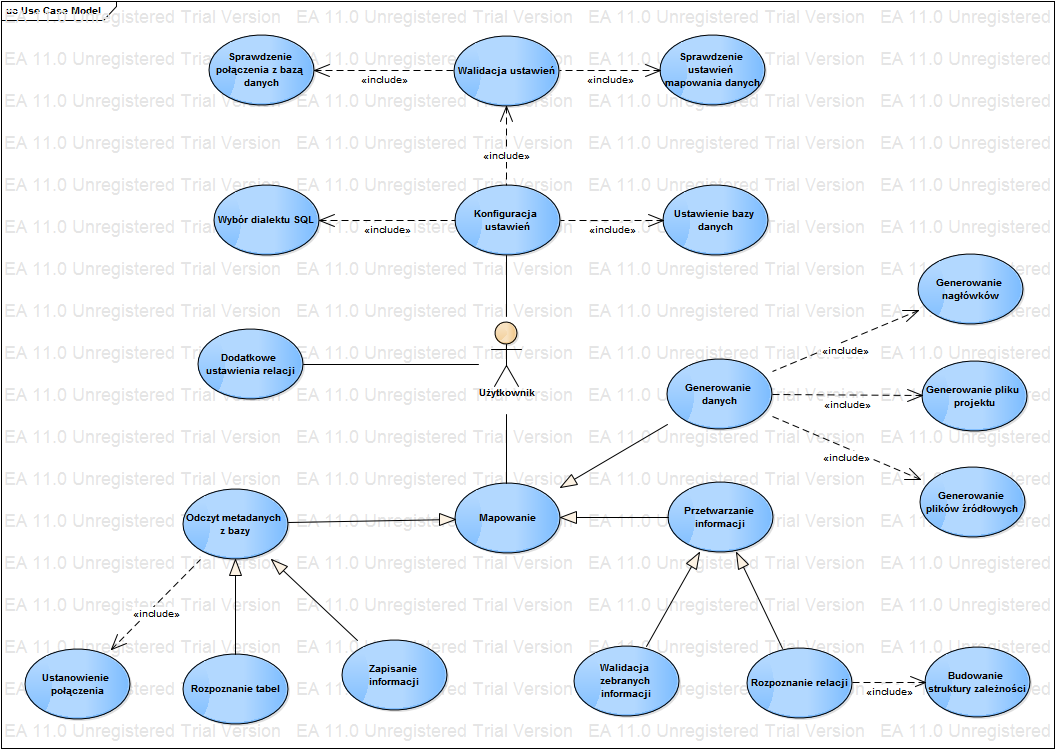
\includegraphics[width=1.4\textwidth, angle=90]{images/QubicUseCase.png}
	\caption{Diagram przypadków użycia modułu generatora.}
\end{figure}
\FloatBarrier

\begin{figure}[h]
	\centering
	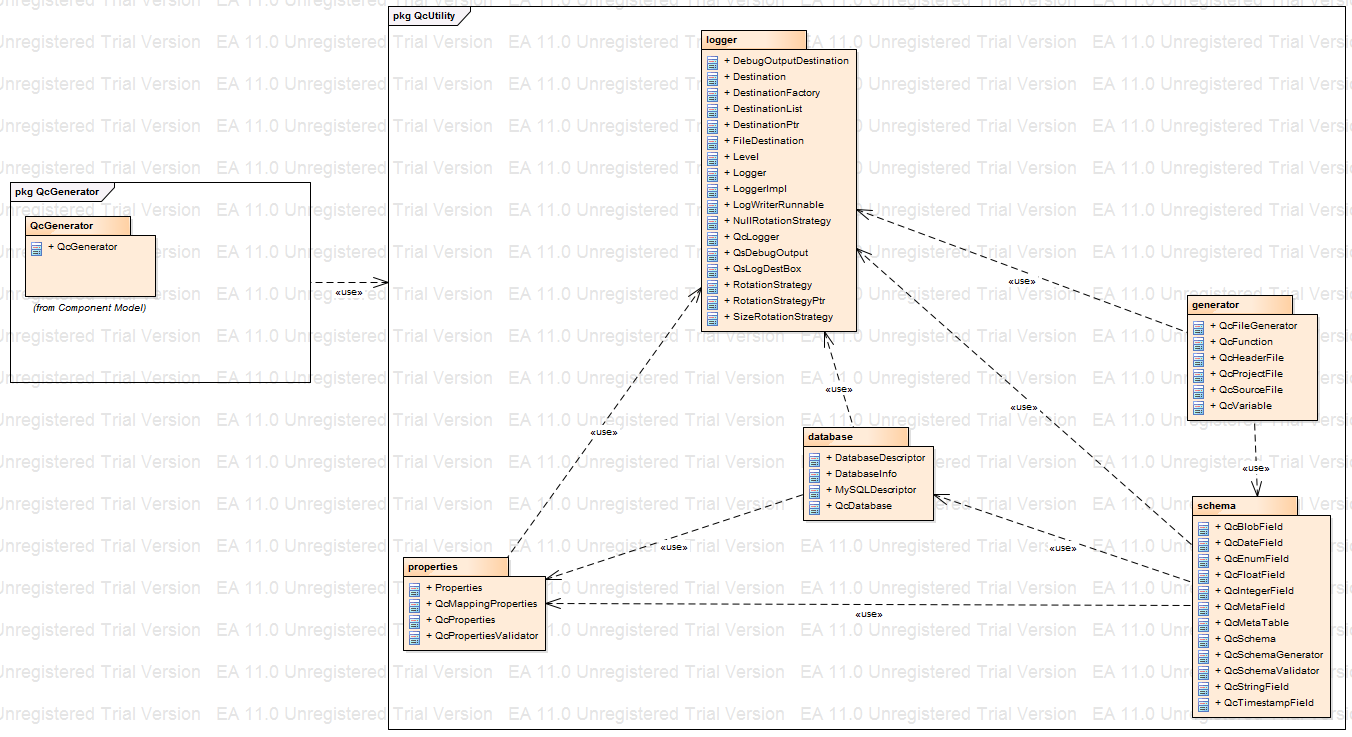
\includegraphics[width=1.4\textwidth, angle=90]{images/Qubic.png}
	\caption{Diagram koncepcyjny generatora.}
\end{figure}
\FloatBarrier

{\color{black} Pakiet QcUtility jest w istocie biblioteką współdzieloną realizującą generowanie opisu mapowania obiektowo-relacyjnego. Moduł QcGenerator natomiast jest aplikacją opartą o funkcjonalność udostępnioną przez bibliotekę. Moduł główny zajmujący się generowaniem został podzielony na logiczne części w celu wyraźnej separacji odpowiedzialności każdego modułu\footnote{Zasada pojedynczej odpowiedzialności mówi że procesy powinny być od siebie niezależne i zaimplementowane w postaci oddzielnych klas lub modułów, które komunikują się ze sobą przy pomocy publicznych interfejsów.}. \\
\indent Pakiet ,,properties'' odpowiada za odczyt i sprawdzanie ustawień aplikacji. Wszy\-stkie ustawienia są sprawdzane przed połączeniem z bazą danych. Kolejny pakiet ,,database'' jest odpowiedzialny za połączenie z bazą danych oraz udostępnienie informacji o strukturze bazy. Informacje te są następnie przekazywane do klasy {\tt QcSchemaGenerator} pochodzącej z pakietu ,,schema''. Kolejnym krokiem jest złożony proces mapowania, który najpierw odczytuje dane z bazy i zapisuje je do pamięci, następnie przeprowadza walidacje zebranych informacji oraz buduje struktury zależności. Ostatnim krokiem jest sam proces generowania projektu gotowego do użycia w środowisku programistycznym, za który odpowiedzialny jest pakiet ,,generator''. \\ \indent Warto również wspomnieć o pakiecie ,,logger''. Jest on używany przez wszystkie inne części aplikacji. Pozwala w prosty i przejrzysty sposób śledzić przebieg procesu mapowania oraz wychwycić ewentualne błędy. Został tu użyty projekt o otwartych źródłach o nazwie QsLog \cite{qslog}. Kryteriami wyboru była łatwa rozszerzalność i prostota użycia. Dzięki temu w prosty sposób można było przekierować logi programu do interfejsu użytkownika zbudowanego w oparciu o aplikację szkieletową Qt. W tym celu dodana została klasa {\tt QsLogDestBox}, która pozwala zapisywać dane do odpowiedniego kontenera Qt. Dodana została również klasa {\tt QcLogger}, która jest nakładką na funkcje udostępniane przez projekt {\tt QsLog} i została stworzona w oparciu o wzorzec singleton\footnote{Singleton - wzorzec projektowy ograniczający możliwość tworzenia obiektów danej klasy do jednej instancji oraz zapewniający globalny dostęp do stworzonego obiektu.}. Formatuje ona w odpowiedni sposób komunikaty aplikacji, zapisuje dane do pliku logowania, który tworzony jest w folderze aplikacji oraz odpowiedzialna jest za ustawienie poziomu logowania komunikatów aplikacji.}
	

\begin{figure}[h]
	\centering
	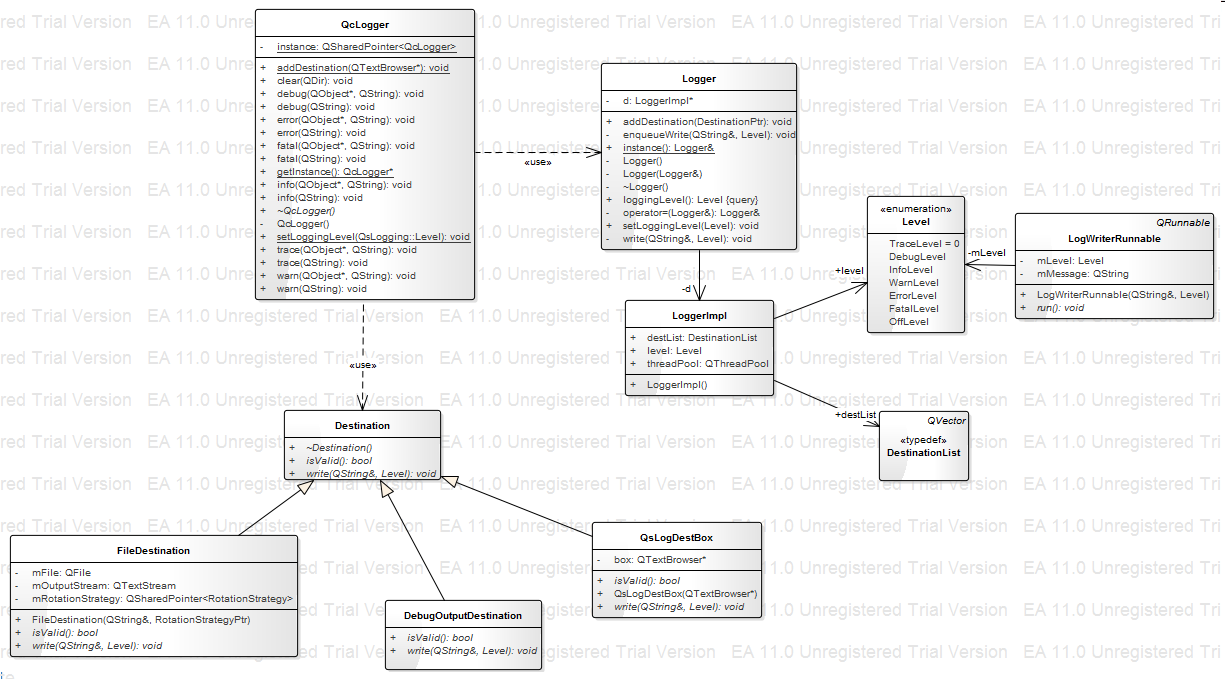
\includegraphics[width=1.4\textwidth, angle=90]{images/logger.png}
	\caption{Diagram klas modułu logera.}
\end{figure}
\FloatBarrier

\begin{figure}[h]
	\centering
	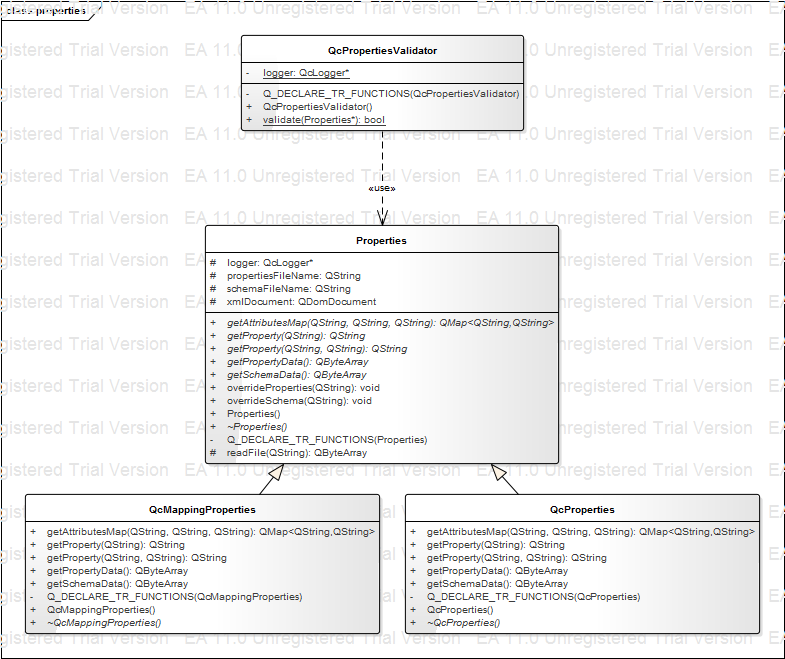
\includegraphics[width=1\textwidth]{images/properties.png}
	\caption{Diagram klas modułu ustawień.}
\end{figure}
\FloatBarrier	

Wszelkie ustawienia potrzebne do połączenia z bazą danych oraz do przeprowadzenia procesu mapowania tabel na klasy są obsługiwane przez powyższy moduł. {\color{black}Klasa {\tt QcMappingProperties} odczytuje informacje z pliku, który przechowuje informacje na jaki typ danych powinna zostać zmapowana odpowiednia kolumna w tabeli. Druga klasa {\tt QcProperties} jest odpowiedzialna za odczytanie informacji do ustanowienia połączenia z bazą danych. Dodatkowo została udostępniona klasa {\tt QcPropertiesValidator}, której zadaniem jest sprawdzenie istnienia i poprawności plików ustawień.}
\newpage
Moduł bazy danych pełni kilka funkcji:
\begin{itemize}
\item{Jest odpowiedzialny za utworzenie połączenia z bazą danych i odczyt metadanych z bazy}
\item{Zbiera informacje o nazwach tabelach, typach danych w tabelach, kluczach głównych, kluczach obcych oraz powiązanych tabelach i przekazuje je do modułu zajmującego się przetwarzaniem tych informacji.}
\item{Dzięki odpowiedniej hierarchii klas zapewnia wsparcie dla różnych systemów baz danych. }
\end{itemize}

Wspierane przez Qubica typy baz danych są ograniczone przez framework Qt. Udostępnia on sterowniki i wsparcie dla następujących baz danych:
\begin{itemize}
\item{IBM DB2}
\item{Borland InterBase}
\item{MySQL}
\item{Oracle Call Interface Driver}
\item{Open Database Connectivity (ODBC) - Microsoft SQL Server and other ODBC-compliant databases}
\item{PostgreSQL}
\item{SQLite version 2}
\item{SQLite version 3}
\item{SQLite version 3 for Symbian SQL Database}
\item{Sybase Adaptive Server Note: obsolete from Qt 4.7}
\end{itemize}

{\color{black} Z wyżej wymienionych języków, aplikacja przewiduje jedynie implementację pozwalającą generować projekt z baz danych typu MySQL. Możliwe będzie natomiast proste rozszerzenie aplikacji o obsługę dodatkowych baz danych. Dokładny opis wraz z przykładem zostanie przedstawiony w dalszej części pracy, w osobnym rozdziale.}

\begin{figure}[h]
	\centering
	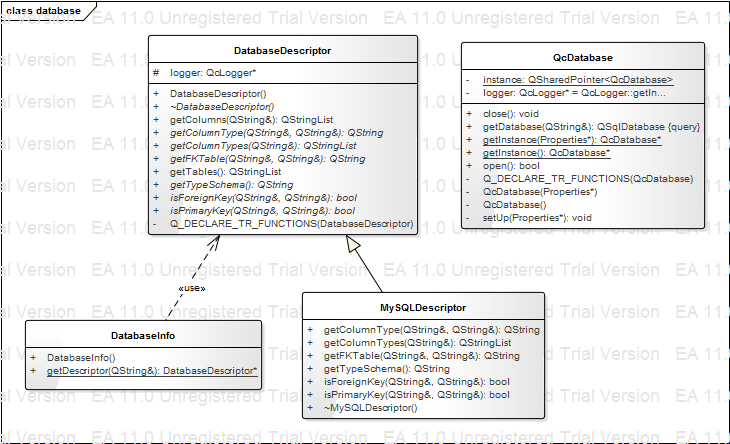
\includegraphics[width=1\textwidth]{images/database.png}
	\caption{Diagram klas modułu bazy danych.}
\end{figure}
\FloatBarrier	

\begin{figure}[h]
	\centering
	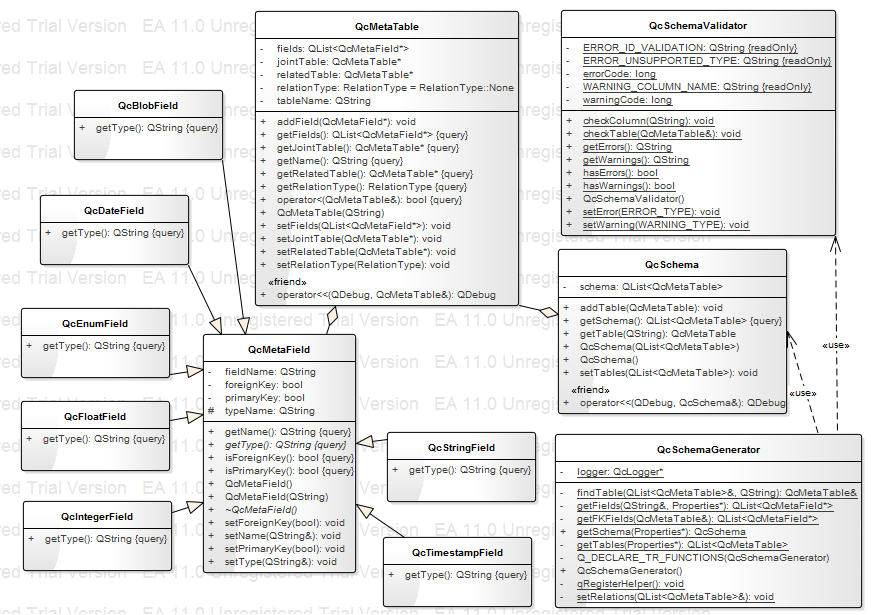
\includegraphics[width=1\textwidth]{images/schema.png}
	\caption{Diagram klas modułu budowania struktury danych.}
\end{figure}
\FloatBarrier	

Powyższy moduł jest najważniejszą częścią aplikacji. Jego zadaniem jest przetworzenie zebranych informacji.
\begin{itemize}
\item{tworzy w pamięci strukturę odczytanych tabel}
\item{automatycznie rozpoznaje relacje między tabelami (jeden do jednego, jeden do wielu), poprzez analizę powiązań między kluczami głównymi i obcymi w tabelach.}
\item{mapuje typy kolumn bazy danych na odpowiednie typy języka}
\item{sprawdza czy zebrane dane spełniają postawione założenia}
\item{udostępnia interfejs generujący}
\end{itemize}

\begin{figure}[h]
	\centering
	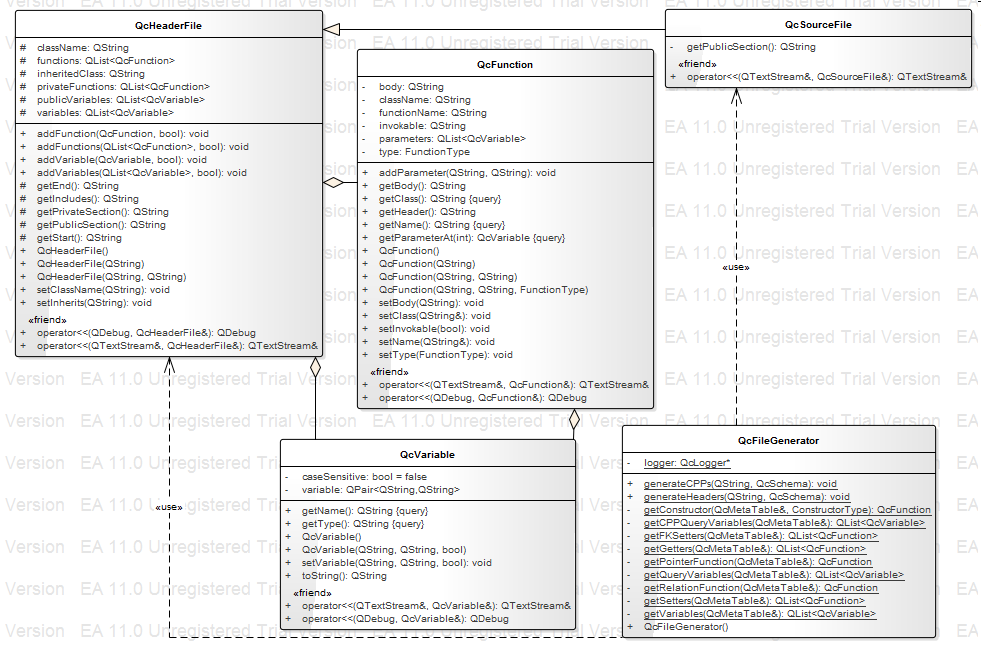
\includegraphics[width=1\textwidth]{images/generator.png}
	\caption{Diagram klas modułu generatora projektu.}
\end{figure}
\FloatBarrier	

Ostatni moduł udostępnia generator plików, który bazując na wygenerowanej strukturze danych tworzy gotowy projekt dla programisty. Wszystkie zebrane informacje są przekształcane w gotowe pliki nagłówkowe i źródłowe języka C++. {\color{black} Z uwagi na budowę plików źródłowych i nagłówkowych języka C++ zostały stworzone klasy reprezentujące zmienne, funkcje oraz same pliki zawierające kod. Wszy\-stkie dane są generowane na podstawie wcześniej zbudowanego schematu bazy i przetwarzane do postaci kodu przez klasę {\tt QcFileGenerator}.}

\section{Implementacja: punkty kluczowe}
W tej części pracy zostaną przedstawione kluczowe fragmenty kodu odpowiadające ze główny przepływ danych przy generowaniu opisu mapowania obiektowo-relacyj\-nego. Główny moduł biblioteki współdzielonej oraz przykładowa aplikacja z interfejsem graficznym wykorzystująca udostępniane przez stworzoną bibliotekę funkcje. \\
	\indent Do połączenia z bazą została użyta klasa zaprojektowana zgodnie z wzorcem projektowym o nazwie singleton.
	
\begin{framed}
\lstinputcplusplus[caption={QcDatabase}]{additional/qcdatabase.h}
\end{framed}

Ważnym krokiem przed przystąpieniem do procesu generowania jest uzyskanie informacji z bazy danych o tabelach, typach kolumn, kluczach głównych i obcych. W celu zapewnienia wsparcia dla różnych systemów relacyjnych baz danych stworzona została klasa abstrakcyjna {\tt DatabaseDescriptor} , którą należy rozszerzyć aby obsłużyć konkretną bazę danych, a następnie dodać wpis do klasy {\tt DatabaseInfo} zajmującej się tworzeniem konkretnej klasy w zależności od używanej bazy danych. Wymusza ona na użytkowniku implementację metod, które udostępnią informacje potrzebne do prawidłowego utworzenia schematu bazy danych w pamięci. {\color{black} Przykład implementacji obsługi bazy danych zostanie opisany w rozdziale zajmującym się możliwościami rozszerzania aplikacji.} Oto przykładowy wpis w klasie {\tt DatabaseInfo} dodający obsługę baz typu MySQL oraz kod klasy {\tt DatabaseDescriptor} pokazujący wymagane metody:

\begin{framed}
\begin{lstlisting}[language=C++]
 if(driverName.contains("MYSQL",Qt::CaseInsensitive)) 
 {
     return new MySQLDescriptor();
 }
\end{lstlisting}
\end{framed}

\begin{framed}
\lstinputcplusplus[caption={DatabaseDescriptor}]{additional/databasedescriptor.h}
\end{framed}

Kolejnym problemem jest odpowiednie mapowanie typów kolumn na typy języ\-ka C++. Rozwiązaniem tego problemu stanowi klasa {\tt QcMetaField}, która jest odpowiednikiem kolumny w tabeli i przechowuje informacje o jej nazwie, typie oraz właściwościach, np. czy jest kluczem głównym. Jest to również klasa abstrakcyjna i w celu zarejestrowania nowego typu, który będzie obsługiwany przez aplikację należy rozszerzyć tą klasę, dodać wpis do funkcji w klasie {\tt QcSchemaGenerator} w celu zarejestrowania klasy w systemie refleksji Qt oraz zarejestrować nowy typ w pliku {\tt qcmapping.xml} zawierającym ustawienia mapowania danych. {\color{black} Przykład zostanie przedstawiony w osobnym rozdziale.}

\begin{framed}
\lstinputcplusplus[caption={QcMetaField}]{additional/qcmetafield.h}
\end{framed}

Tak wygląda przykładowy wpis w pliku mapowań, który typ {\tt char} bazy danych mapuje na obiekt {\tt QcStringField}. 

\begin{framed}
\begin{lstlisting}[language=XML]
<qc:map fromType="char" toType="QcStringField"/>
\end{lstlisting}
\end{framed}

Jedna z najważniejszych klas modułu generatora to klasa {\tt QcSchemaGenerator}, która  wykorzystuje wyżej opisane klasy w celu utworzenia struktury bazy w pamięci programu. {\color{black} Klasa {\tt QcMetaTable} reprezentuje pojedynczą tabelę bazy danych. Przechowuje ona nazwę tabeli, informacje o nazwach kolumn w tabeli, ich typach, kluczach obcych oraz typie relacji między daną tabelą, a tabelą powiązaną kluczem obcym. Główna funkcja {\tt getTables} jest odpowiedzialna za odczytanie tabel, nazw i typów kolumn oraz rozpoznanie relacji między tabelami. W trakcie przetwarzania wykonywana jest również walidacja danych przez klasę {\tt QcSchemaValidator}. Sprawdza ona czy każda tabela posiada własny klucz główny. Najkosztowniejszą operacją jest automatyczne wykrycie relacji między tabelami. W tym celu sprawdzana jest najpierw ilość kluczy obcych w danej tabeli. W przypadku znalezienia jednego klucza obcego, szukana jest tabela powiązana i w obu zapisywane są wskaźniki do drugiej tabeli wraz z informacją o rozpoznaniu relacji typu jeden do wielu.\\
\indent W przypadku znalezienia dwóch kluczy obcych w tabeli, program zakłada, że tabela ta jest tabelą łącznikową. Wyszukiwane są obie powiązane tabele i w każdej z nich zapisywane są wskaźniki do dwóch pozostałych tabel, wraz z informacją o rozpoznaniu relacji typu wiele do wielu. W przypadku tej relacji została dodana również możliwość wskazania, które relacje typu wiele do wielu mają zostać wzięte pod uwagę przy generowaniu projektu.}

\begin{framed}
\lstinputcplusplus[caption={QcSchemaGenerator}]{additional/qcschemagenerator.cpp}
\end{framed}

Na podstawie utworzonej struktury danych generowane są pliki projektu. Ze względu na wymagany podział projektu na pliki źródłowe i nagłówkowe została utworzona odpowiednia struktura klas. Najbardziej szczegółowa {\tt QcVariable} reprezentuje zmienną i przechowuje informacje o jej nazwie i typie. Kolejne klasy reprezentują konkretne metody w klasie ({\tt QcFunction}), pliki źródłowe ({\tt QcHeader\-File}) i nagłówkowe ({\tt QcSourceFile}). Ciała funkcji i nazwy metod zostały narzucone przez drugą część pracy zajmującą się mapowaniem obiektowo-relacyjnym. Generowane są m.in. konstruktory, nagłówki, klasy, funkcje odczytujące i ustawiają\-ce zmienne reprezentujące kolumny w bazie danych czy funkcje pozwalające uzyskać obiekt powiązanej klasy. {\color{black} Zbudowany w pamięci model plików źródłowych i nagłówkowych zostaje następnie zapisany do fizycznych plików na dysku użytkownika.}

\begin{framed}
\lstinputcplusplus[caption={QcFileGenerator}]{additional/qcfilegenerator.h}
\end{framed}

\section{Opis użytkowania aplikacji}

Proces generowania i korzystania z gotowego projektu jest bardzo prosty i wiąże się z wykonaniem kilku kroków.

\begin{itemize}
\item W podfolderze {\tt resources} aplikacji znajdują się dwa pliki ustawień \\{\tt qcmapping.xml} oraz {\tt qcproperties.xml}. Przed rozpoczęciem generowania należy uzupełnić informacje o bazie w drugim pliku.
\item Po uruchomieniu aplikacji należy w {\tt Menu -> Load} załadować pliki ustawień. Są one domyślnie zczytywane z folderu {\tt resources} oraz sprawdzane pod kątem błędów.
\item Następnym krokiem jest ustanowienie połączenia z bazą, {\tt Menu -> Connect}. 
\item Jeśli poprzedni krok został wykonany, dostępne będą opcje generowania oraz ustawienia dodatkowych informacji o relacjach.
\subitem {\tt Menu -> Set Relations} pozwala na zdefiniowanie, które relacje wiele do wielu zostaną uwzględnione przy generowaniu projektu.
\subitem {\tt Menu -> Generate} - po wybraniu tej opcji, program spyta nas o podanie folderu, w którym zostanie wygenerowany projekt.
\end{itemize}

Po wygenerowaniu projektu można zacząć tworzenie aplikacji opartej o Qubica. W celu późniejszego uruchomienia stworzonej aplikacji wymagane są następujące kroki:

\begin{itemize}
\item Z folderu z wygenerowanym projektem należy skopiować plik {\tt qb.proper\-ties} do folderu z plikiem wykonawczym tworzonej aplikacji {\color{black} Jest on wymagany przez drugą część aplikacji do działania.}
\item Do folderu ze stworzoną aplikacją należy również skopiować bibliotekę z odpowiednim sterownikiem bazy danych dla języka C++. {\color{black} Aplikacja szkieletowa Qt wymaga jej w celu nawiązania połączenia z bazą danych.}
\end{itemize}

 Cała część zajmująca się mapowaniem obiektowo-relacyjnym została wbudowana w stworzoną bibliotekę, dzięki czemu nie wymaga to dodatkowego nakładu w postaci ściągania i ustawiania czegokolwiek.

{\color{black}
\section{Przykład użycia generatora opisu}
Przykład zostanie oparty o testową bazę danych, która została przedstawiona w rozdziale \ref{sec:database}. Zawiera ona podstawowe relacje typu jeden do wielu oraz wiele do wielu, co pozwala na testowanie wszystkich funkcjonalności generatora. \\
\indent Poniżej przedstawiony jest interfejs prostej aplikacji graficznej opartej o funkcje udostępniane przez stworzoną bibliotekę. Została ona stworzona jedynie jako reprezentacja możliwości stworzonej biblioteki. Odczytuje ona i sprawdza poprawność odpowiednich plików ustawień, tj. pliku mapowań oraz pliku z informacjami o połączeniu. Następnie po poprawnej walidacji ustawień pozwala na ustanowienie połączenia z bazą. \\
\indent Pierwszym krokiem jest dostosowanie plików ustawień znajdujących się w folderze {\tt resources}. Plik {\tt qcproperties.xml} przechowuje informacje potrzebne do połączenia z bazą danych. Drugi plik {\tt qcmapping.xml} służy do mapowania typów kolumn na typy języka C++, a jego zastosowanie zostanie przedstawione w następnym rozdziale. Po uruchomieniu aplikacji należy z menu wybrać opcje {\tt Load -> Database properties}, a następnie {\tt Load -> Mapping proper\-ties}. Pliki ustawień zostaną odczytane i sprawdzona zostanie ich poprawność.

\begin{figure}[h]
	\centering
	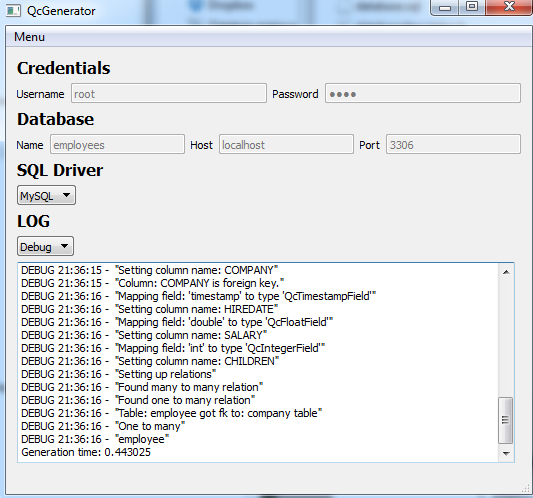
\includegraphics[width=.8\textwidth]{images/qubic-gen.png}
	\caption{Interfejs generatora.}
\end{figure}
\FloatBarrier	

Dodatkowo została dodana możliwość zdefiniowania przez użytkownika, które relacje wiele do wielu mają zostać uwzględnione przy generowaniu projektu. Służy do tego opcja {\tt Set Relations} w menu aplikacji. Interfejs zostaje dostosowany w zależności od ilości wykrytych relacji tego typu. Zostawienie pustego pola jest równoznaczne z usunięciem generowania funkcji odpowiedzialnej za obsługę danej relacji wiele do wielu.

\begin{figure}[h]
	\centering
	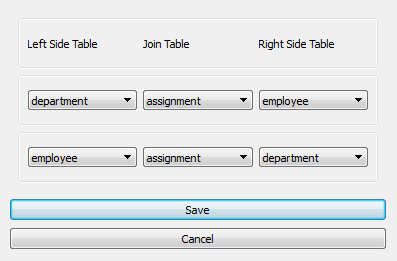
\includegraphics[width=1\textwidth]{images/qubic-rel.png}
	\caption{Interfejs generatora.}
\end{figure}
\FloatBarrier	

Najważniejszą funkcją jest oczywiście możliwość wygenerowania projektu jeśli wcześniejsze kroki zostaną wykonane bez błędów. Po wybraniu opcji {\tt Generate} aplikacja zapyta nas w jakim folderze zapisać wygenerowany projekt. Wygenerowane pliki znajdziemy w folderze {\tt Qubic-Generated}. Są one podzielone na dwie części. Moduł zajmujący się mapowaniem obiektowo-relacyjnym znajduje się w folderze {\tt ORM}, natomiast wygenerowane klasy, w folderze {\tt Generated}. Dodatkowo załączony został plik ustawień {\tt qb.properties} wymagany później do działania przez aplikacje stworzoną w oparciu o Qubica. 

\begin{figure}[h]
	\centering
	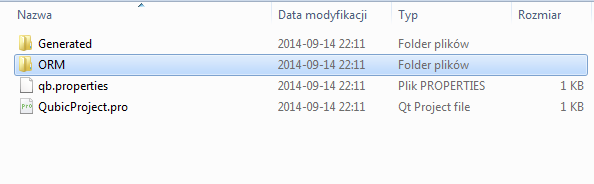
\includegraphics[width=1\textwidth]{images/qubic-out.png}
	\caption{Struktura stworzonego projektu.}
\end{figure}
\FloatBarrier	

Poniżej przedstawione pliki, nagłówkowy i źródłowy zostały stworzone w oparciu o tabelę {\tt Department}, która reprezentuje dział firmy. Jest ona powiązana relacją wiele do wielu z tabelą {\tt Employee} reprezentującą pracownika. Jak widać wygenerowana została odpowiednia funkcja {\tt getEmployees}, która pozwoli uzyskać odpowiednich pracowników z danego działu. 

\begin{framed}
\lstinputcplusplus[caption={QcSchemaGenerator}]{additional/department.h}
\end{framed}

\begin{framed}
\lstinputcplusplus[caption={QcSchemaGenerator}]{additional/department.cpp}
\end{framed}

\section{Możliwości rozszerzania aplikacji}

Dzięki stworzeniu odpowiedniej hierarchii klas i użyciu możliwości programowania obiektowego, można w łatwy sposób dodać do aplikacji obsługę nowego typu bazy danych, czy typu kolumny w tabeli. W celu dodania obsługi nowego typu bazy danych należy:

\begin{enumerate}
\item{Stworzyć klasę dziedziczącą z klasy {\tt DatabaseDescriptor} i zaimplementować metody: {\tt getColumnType, getColumnTypes, getFKTable,}\\ {\tt getTypeSchema, isForeignKey, isPrimaryKey}.}
\subitem{1.1. {\tt getColumnType} - na podstawie nazwy tabeli i nazwy kolumny zwraca typ kolumny.}
\subitem{1.2. {\tt getColumnTypes} - na podstawie nazwy tabeli zwraca listę typów kolumn w tej tabeli.}
\subitem{1.3. {\tt getFKTable} - na podstawie nazwy tabeli i nazwy kolumny klucza obcego zwraca nazwę powiązanej tabeli.}
\subitem{1.4. {\tt getTypeSchema} - zwraca nazwę bazy danych, w której znajdują się informacje o strukturze bazy, z której chcemy wygenerować projekt.}
\subitem{1.5. {\tt isForeignKey, isPrimaryKey} - na podstawie nazwy tabeli i nazwy kolumny zwraca informacje czy jest ona kluczem obcym lub kluczem głównym.}
\item{Dodać wpis do klasy {\tt DatabaseInfo} rejestrujący stworzoną klasę dla odpowiedniego typu bazy danych. Przykładowa linijka kodu dla bazy MySQL znajduje się poniżej.}
\end{enumerate}

\begin{framed}
\begin{lstlisting}[language=C++]
 if(driverName.contains("MYSQL",Qt::CaseInsensitive)) 
 {
     return new MySQLDescriptor();
 }
\end{lstlisting}
\end{framed}

Oto fragment kodu z klasy {\tt MySQLDescriptor} pokazujący implementacje funkcji {\tt getColumnType}.

\begin{framed}
\lstinputcplusplus[caption={QcSchemaGenerator}]{additional/mysqldescriptor.cpp}
\end{framed}

Oprócz dodawania obsługi innych typów baz danych, użytkownik może również dodać obsługę nowych typów danych istniejących w bazie. W tym celu należy:

\begin{enumerate}
\item{Dodać wpis do pliku {\tt qcmapping.xml} mapujący typ w bazie danych na odpo\-wiednią klasę.}
\item{Jeśli klasa do obsługi danego typu nie istnieje należy stworzyć klasę dziedzi\-czącą z klasy {\tt QcMetaField} i nadpisać jedną metodę {\tt getType}. Zwraca ona nazwę typu języka C++, np. ,,int'',  który ma zostać użyty jeśli zostanie znaleziony odpowiedni typ kolumny w czasie generowania.}
\item{Ostatnim krokiem jest dodanie wpisu do nagłówka klasy {\tt QcSchemaGenerator}, który pozwoli rozpoznać nowy typ w systemie refleksji Qt. Dzięki temu jeśli dodany zostanie nowy typ, obsługiwany przez już istniejące klasy, nie będzie wymagana ponowna kompilacja aplikacji.}
\end{enumerate}

Przykładowa implementacja funkcji {\tt getType} dla typu {\tt blob}.

\begin{framed}
\begin{lstlisting}[language=C++]
QString QcBlobField::getType()const {
    return "QByteArray";
}
\end{lstlisting}
\end{framed}

Wpis w pliku {\tt qcmapping.xml} rejestrujący powyższy typ.

\begin{framed}
\begin{lstlisting}[language=XML]
<qc:map fromType="blob" toType="QcBlobField"/>
\end{lstlisting}
\end{framed}

Wpis w nagłówku klasy {\tt QcSchemaGenerator} dodajemy do funkcji \\{\tt qRegisterHelper}.

\begin{framed}
\begin{lstlisting}[language=C++]
template<>
void QcSchemaGenerator::qRegisterHelper<QcMetaField>()
{
    qRegisterMetaType<QcStringField>();
    qRegisterMetaType<QcIntegerField>();
    qRegisterMetaType<QcEnumField>();
    qRegisterHelper<QcFloatField>();
    qRegisterHelper<QcTimestampField>();
    qRegisterHelper<QcDateField>();
    qRegisterHelper<QcBlobField>();
}
\end{lstlisting}
\end{framed}

}
\chapter{Podsumowanie}
Ten rozdział zawiera podsumowanie pracy oraz uzyskanych wyników. Omówione zostają dodatkowe możliwości rozwoju tematu jak i całej aplikacji Qubic.
\section{Dyskusja wyników}
 Głównym atutem stworzonej aplikacji jest wsparcie większej ilości dialektów SQL od konkurencyjnych rozwiązań oraz bardzo mała ilość podobnych aplikacji w języku C++, dzięki czemu Qubic staje się bezkonkurencyjnym rozwiązaniem w swojej dziedzinie. Dodatkowym czynnikiem, dzięki któremu stworzona aplikacja staje się lepszym wyborem jest brak opłat za jej użytkowanie. Prostota użycia, brak zależności od zewnętrznych aplikacji czy dodatkowego ręcznego konfigurowania to tylko kilka z wielu atutów stworzonego generatora opisu mapowania obiektowo-relacyjnego.
\section{Ocena możliwości wdrożenia Qubica}
Qubic pozwala zaoszczędzić programistom dużą ilość czasu w fazie tworzenia aplikacji, dzięki czemu mogą sie oni skupić na innych częściach projektu. Moduł generujący warstwę dostępu do danych jest prosty i szybki w użyciu oraz dalszym rozwoju. W razie potrzeby jest prosto konfigurowalny, a dzięki generycznej budowie aplikacja może być łatwo dostosowywana do własnych potrzeb. Dzięki temu jej wdrożenie nie wiąże się z dużymi kosztami, a pozwala na późniejsze zaoszczędzenie cennego czasu w fazie implementacyjnej.
\section{Perspektywy dalszego rozwoju}
Dodatkowym atutem stworzonej aplikacji byłby moduł zajmujący się procesem odwrotnym, czyli generowaniem bazy danych z istniejącego schematu obiektów klas lub pliku tworzącego bazę danych. Pozwoliłoby to na pewną swobodę programistom, których zadaniem jest stworzenie bazy, a łatwiejsze jest dla nich stworzenie struktury w języku programowania niż bezpośrednie tworzenie bazy danych używając języka SQL.
\addcontentsline{toc}{chapter}{Bibliografia} 
\begin{thebibliography}{99}
	\bibitem{ejb} {M. Keith, M. Schincariol, Pro EJB 3 Java persistence API. APress, 2006. ISBN-13 978-1-59059-645-6}
	\bibitem{hibernateInAction} {C. Bauer, G. King, Hibernate w akcji, Helion, 2007, ISBN: 978-83-246-0527-9}
	\bibitem{c++patterns} {A. Ezust, P. Ezust, Introduction to Design Patterns in C++ with Qt, Pearson Education, Inc, 2012 , ISBN 978-0-13-282645-7}
	\bibitem{c++2} {D. Gennaro, Advanced C++ Metaprogramming, CreateSpace Independent Publishing Platform , 2011, ISBN-13 978-1460966167}
	\bibitem{sql} {P. Wilton, J. Colby, Beginning SQL, Wrox, 2005, ISBN 0-7645-7732-8}
	\bibitem{mysqlweb} {http://dev.mysql.com/doc/refman/5.6/en/ - [dostęp 05.08.2014]}
	\bibitem{strostrup} {http://www.stroustrup.com/C++11FAQ.html - [dostęp 10.08.2014]}
	\bibitem{qtframework} {http://qt-project.org/ - [dostęp 07.01.2014]}
	\bibitem{dll} {http://msdn.microsoft.com/en-us/library/windows/desktop/ms681914(v=vs.\\85).aspx - [dostęp 29.07.2014]}
	\bibitem{hibernateweb} {http://docs.jboss.org/hibernate/orm/4.3/manual/en-US/html/\\- [dostęp 02.08.2014]}
	\bibitem{jooqweb} {http://www.jooq.org/javadoc/3.4.x/ - [dostęp 02.08.2014]}
	\bibitem{qslog} {https://bitbucket.org/razvanpetru/qt-components/src/a476515a5b40479da3\\e90e18557bbc0257dbda16/QsLog/?at=default - [dostęp 12.09.2014]}
	%wzorce
	\bibitem{mvc} {http://msdn.microsoft.com/en-us/library/ff649643.aspx - [dostęp 28.07.2014]}
	\bibitem{dao} {http://www.oracle.com/technetwork/java/dataaccessobject-138824.html - [dostęp 28.07.2014]}
	\bibitem{datalayer} {http://msdn.microsoft.com/en-us/library/ee658127.aspx - [dostęp 27.07.2014]}
	%obrazki
	\bibitem{ormimg} http://www.visual-paradigm.com/VPGallery/img/orm/Overview/ORM-Overview.png --  [dostęp 02.11.2013]
	\bibitem{c++testimg} http://blog.famzah.net/2010/07/01/cpp-vs-python-vs-perl-vs-php-performance-benchmark/ - [dostęp 02.07.2014]
	\bibitem{dllimg} {http://i.msdn.microsoft.com/dynimg/IC34006.gif - [dostęp 29.07.2014]}
	\bibitem{qxentity} {http://www.qxorm.com/qxentityeditor/resource/qxee\_sample.png - [dostęp 04.09.2014]}
\end{thebibliography}

\addcontentsline{toc}{chapter}{Spis rysunków} 
\listoffigures

\addcontentsline{toc}{chapter}{Spis tabel} 
\listoftables

\end{document}
